% Use class option [extendedabs] to prepare the 1-page extended abstract.
\documentclass[extendedabs]{bmvc2k}
\usepackage[colorlinks = true,
            linkcolor = blue,
            urlcolor  = blue,
            citecolor = blue,
            anchorcolor = blue]{hyperref}
\usepackage{kotex}
% for the fancy \koTeX logo
\usepackage{kotex-logo}

% Document starts here
\begin{document}


\title{YOLO pre-report}
\addauthor{
김태훈$^{1}$
}{}{1}

\addinstitution{
$^1$부산대학교 전기컴퓨터공학부.  
}
 
\maketitle
\noindent



\section{Introduction}
YOLO\cite{yolopaper} is the object detection with unified architecture, which predicts bounding boxes and class probabilities from full images in one evaluation. 

Unlike object detection with sliding window and region-proposal based architectures, YOLO is extremely fast(45 frames per second) and better at generalizing from natural images to other domain, which means a model that learns from natural images can detect objects from other domain like artworks. Also, YOLO makes less background errors but more localization errors compared to Fast R-CNN\cite{fastrcnn}

This report summarize the YOLO paper\cite{yolopaper} focusing on the architectures.

\section{Unified Detection}
YOLO network uses features from entire images to predict each bounding box. This design enable end-to-end training and real-time speed.

This system divides the input image into an $S\times S$ grid. Each grid cell predicts $B$ bounding boxes and confidence scores for those boxes. These confidence scores means how confident the model is that the box contains an object and also how accurate it thinks the box is that it predicts. Confidence is defined as $Pr(Object) \times IOU^{truth}_{pred}$. IOU means that Intersection over Union of ground-truth bounding boxes and predicted bounding boxes.

Each bounding box contains $x,y,w,h$. $(x,y)$ coordinates is center of the box relative to the grid cell, and $(w,h)$ is width and height relative to the whole image.

Each grid cell also predicts $C$ conditional class probabilities, which means the probabilities are conditioned on the grid cell containing an object, $PR(Class_i | Object)$. Also, each grid cell predicts one set of class probabilities regardless of the number of boxes.

Finally, These predictions are encoded as an $S\times S \times (B*5+C)$ tensor with $S\times S$ grid that divided from images, $B$ bounding boxes and $C$ class probabilities that each grid cell predicts.

\section{Network Design}
This network contains 24 convolutional layers followed by 2 fully connected layers. The convolutional layers extract features from image and the fully connected layers predict the class probabilities and coordinates of bounding boxes. Fast YOLO uses fewer convolutional layers(9 instead of 24) for fast object detection.

\section{Training} \label{training}
The first 20 convolutional layers was pretrained with Imagenet datasets. For pretraining, the convolutional layers followed by a average-pooling layer and a fully connected layer used. Then, four convolutional layer and two fully connected layers are added to pretrained network.

They use leaky-ReLU for activation, and sum-of-squares for error function. Unlike normal sum-of-squares function, They increase the loss from bounding box coordinate prediction and decrease the loss from confidence prediction for boxes that don't contain objects because localization is more difficult than classification and there are less grid cells that contains object than those that don't. If normal sum-of-squares function is used, The model can predict all confidence score of grid cell to almost zero.

Also, they predict the square root of the bounding box width and height to reflect more loss for deviation of small boxes. For square root function, the rate of increase decreases as the width and height increase.

YOLO predicts multiple bounding boxes per grid cell, but finally, The bounding boxes that has highest IOU is assigned to be responsible for object. However, some objects can be localized by multiple cells. It can be fixed by non-maximum suppression.
\subsection{Loss Function}
The loss function for training YOLO is figure \ref{lossfunction}. $\mathbf{1}^{obj}_i$ denotes whether object appears in cell $i$, $\mathbf{1}^{obj}_{ij}$ denotes that the $j$th bounding box predictor in cell $i$ is responsible, $\lambda_{noobj} $ denotes balancing parameter for boxes that contain object and those don't, and $\lambda{coord}$ denotes balancing parameter for coordinates loss and classification loss. The meanings of each term are as follows:
\begin{enumerate}
    \item For the responsible bounding box predictor $j$ in cell $i$ (the cell $i$ contains object), get loss of x and y
    \item For the responsible bounding box predictor $j$ in cell $i$ (the cell $i$ contains object), get loss of $\sqrt{w}$ and $\sqrt{h}$. For reflecting deviation of small boxes more, calculate loss of square root (\ref{training})
    \item For the responsible bounding box predictor $j$ in cell $i$ (the cell $i$ contains object), get loss of confidence score $(C_i=1)$
    \item For the bounding box predictor $j$ in cell $i$ (the cell $i$ \textbf{doesn't} contain object), get loss of confidence score $(C_i=0)$
    \item For cell that contains object, get loss of conditional class probability (for correct class, $p_i(c)=1$)
\end{enumerate}

\begin{figure}[t]
	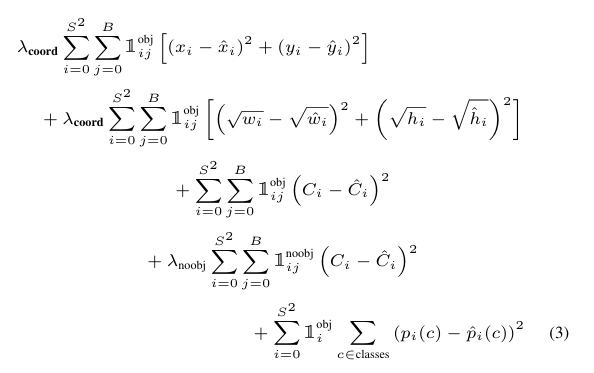
\includegraphics[width=\linewidth]{images/loss.PNG}
	\caption{
		The loss functions for YOLO}
	\vspace{-2mm}
 \label{lossfunction}
\end{figure}

\section{Experiments}
In short, mAP and FPS of YOLO is 63.4 and 45. Also, mAP and FPS of Fast YOLO is 52.7 and 155. For comparision, Faster R-CNN\cite{fasterrcnn} VGG-16 has 73.2 mAP and 7 FPS. the mAP of YOLO isn't biggest, but it is fast and can be processed in real-time.

\section{Conclusion}
YOLO is simple but fast and accurate. Also, YOLO can detect a new image that not in training set. It is fast so it can process in real-time. Therefore, it is useful for application that fast, robust object detection.

\newpage
\bibliography{egbib}

\end{document}
